% =====================================================================
% SCAFFOLD for the camera-ready ("Not All Instructions Are Forgotten Equal").
% Structure + figures/tables placed; PROSE LEFT TO THE AUTHOR.
% Each `% -` line is a bullet of WHAT to say (+ the number to cite), not the
% sentence itself. Write the prose between the bullets, then delete the bullets.
% Numbers below are the v1 (camera-ready) values; verify against paper.pdf.
% =====================================================================
\documentclass{llncs}
\usepackage[T1]{fontenc}
\usepackage{graphicx}
\usepackage{amsmath}
\usepackage{amssymb}
\usepackage{booktabs}
\usepackage{microtype}
\usepackage[htt]{hyphenat}
\emergencystretch=1.5em
\graphicspath{{figures/}}
\usepackage[style=apa]{biblatex}
\addbibresource{references.bib}

\begin{document}

\title{Not All Instructions Are Forgotten Equal}
\titlerunning{Not All Instructions Are Forgotten Equal}
\author{Tom\'as P. Korenblit\orcidID{0009-0002-5682-8475}}
\authorrunning{T. P. Korenblit}
\institute{Universidad Nacional de San Mart\'in, Buenos Aires, Argentina\\
\email{tomaskorenblit@gmail.com}}
\maketitle

% ---------------------------------------------------------------------
\begin{abstract}
% Cover, in order, one tight paragraph (~150-180 words):
% - hook: LLMs lose adherence to user-stated preferences over long conversations.
% - the twist even when system prompt unchanged -> the loss has no visible trigger.
% - central finding: they do NOT forget all instructions equally (per-instruction
%   heterogeneity). Avoid "decay rates" (design is a snapshot, not a curve).
% - the split: most followed by default; a few only when stated; one slightly
%   negative = likely measurement artifact.
% - method, one sentence: planted preferences, multi-turn coding sessions, 3
%   open-source Python codebases, several models, 12 instruction types,
%   deterministic checkers (no LLM judge) -> reproducible; Bayesian hierarchical
%   ordered-logit estimates per-instruction retention.
% - payoff: only 3 of 12 worth restating -> targeted, not blanket, reinforcement.
% - AIS stake (one sentence): agents deployed in loops, no human per step;
%   guardrails are instructions too -> silent decay, nothing flags it without
%   per-instruction monitoring.
\keywords{instruction retention \and context rot \and Bayesian inference
\and AI safety \and LLM evaluation}
\end{abstract}

% --- SPANISH TITLE + RESUMEN (JAIIO requires it for an EN paper) ---
\begin{center}
\vspace{1cm}
{\Large \bfseries\boldmath No Todas las Instrucciones se Olvidan Igual}
\vspace{0.5cm}
\end{center}
\begin{abstract}
% Faithful translation of the EN abstract above. Keep 150-250 words.
% Avoid anglicism drift; keep numbers identical to the EN version.
\keywords{retenci\'on de instrucciones \and degradaci\'on de contexto
\and inferencia bayesiana \and seguridad de la IA \and evaluaci\'on de LLMs}
\end{abstract}

% ---------------------------------------------------------------------
\section{Introduction}
\label{sec:intro}
% Para 1 - the threat model / phenomenon:
% - LLMs deployed as agents that run in loops, call tools, act over hundreds of
%   turns with no human reviewing each step.
% - what governs an agent = its instructions (limits + guardrails), given once,
%   must hold the whole run.
% - adherence erodes as context grows = "context rot". Cite Laban et al. 2025:
%   average 39% compliance drop across 15 models, multi-turn.
% - cause is architectural: non-uniform attention, middle < boundaries
%   (cite liu2024, chowdhury2026). An instruction stated once, buried under tool
%   output; in a loop no user restates it.
%
% Para 2 - safety before cost (KEEP THIS TIGHT; do NOT inflate):
% - chat user notices a dropped preference and restates it; a deployed agent has
%   no supervisor -> guardrail decays silently while the agent acts (irreversible
%   tool effects). Cite mu2025.
% - repeating every instruction each turn: costs tokens, still can't say which
%   constraint holds.
% - safety is conjunctive -> an aggregate compliance rate hides whether the ONE
%   rule that matters lapsed.
%
% Para 3 - the gap:
% - no prior work measures heterogeneity at the individual-instruction level;
%   existing work reports mean compliance (laban2025, he2024) or uniform
%   mitigation (dongre2025).
% - if instructions are retained unequally, the mean hides what a reinforcement
%   policy would act on (already-retained needs none; harmed should get none).
%
% Para 4 - the BKT framing:
% - Bayesian Knowledge Tracing (corbett1994): per-concept mastery from responses.
% - we adapt it: model = student, instructions = concepts. Test via Bayesian
%   ordered-logit with hierarchical per-decision effects on multi-turn coding data.
%
% Para 5 - the three findings (state with numbers; HEDGE 2 and 3):
% - (1) heterogeneity large: treatment effects -2.4 to +5.4 log-odds,
%   sigma_beta = 2.1. (optionally gloss log-odds inline = "a scale for comparing
%   probabilities" -- the one good Grammarly idea.)
% - (2) one type (dependencies_no_new) marginal negative; 94% HDI barely excludes
%   zero -> read as LIKELY MEASUREMENT ARTIFACT, not robust harm.
% - (3) within this design, model + codebase explain little variance; baseline is
%   single-model so frame as model-invariance WITHIN design, not absence of effects.

% ---------------------------------------------------------------------
\section{Related work}
\label{sec:related}
% Para A - degradation in long contexts: laban2025 (39% drop); he2024 (accuracy
%   falls within 3 turns); du2025 (bigger window doesn't fix it). None asks about
%   per-instruction differences.
% Para B - positional attention: liu2024 (U-shaped curve); mu2025 (saturation).
% Para C - uniform mitigation: dongre2025 (periodic reminders); leviathan2025
%   (repetition); note repetition can be counterproductive for some instructions.
% Para D - BKT: corbett1994; 30+ years of per-concept mastery; the analogy.

% ---------------------------------------------------------------------
\section{Method}
\label{sec:method}

\subsection{Decision planting}
% - simulate a coding assistant over 25 turns; inject real source files turns 0-19
%   to build context pressure.
% - treatment: 12 coding preferences as casual inline user requests; 6 early
%   (turns 1-7), 6 late (turns 14-19); span code style, architecture, testing,
%   naming, dependencies, documentation. Give the NumPy-broadcasting example.
% - baseline: identical, nothing planted -> spontaneous compliance.
% - test turns 20-25; each probes 2 decisions (one early, one late).

\subsection{Compliance measurement}
% - deterministic checker per decision, regex/pattern, NO LLM in the loop ->
%   reproducible.
% - ordinal 0-3 (0 = ignored ... 3 = fully followed); say what 1/2 mean.
% - name a couple of checkers (parametrize, broadcasting, no_new_imports).

\subsection{Bayesian model}
% - hierarchical ordered-logistic (cumulative link), per decision type.
% - the equation (keep as display math):
\[ \eta_i = \alpha_{d[i]} + \beta_{d[i]} \cdot \mathrm{treatment}_i \]
% - alpha_d = per-decision baseline, beta_d = per-decision treatment effect, both
%   non-centered hierarchical priors.
% - key parameter = sigma_beta (group-level SD of treatment effects).
% - priors: mu_alpha ~ N(0,1.5), mu_beta ~ N(0,1), sigma ~ Exp(1); offset
%   cutpoints c1 ~ N(0,1.5), dc ~ Exp(1).
% - why drop the full (per-model/codebase) model: near-zero variance
%   (sigma_model, sigma_codebase ~ 0.3); report the simpler per-decision model;
%   diagnostics clean (0 divergences, R-hat <= 1.01, min ESS = 1311).
% - PyMC, NUTS via nutpie, 4 chains x 1000 draws + 1000 tune.

% ---------------------------------------------------------------------
\section{Experimental setup}
\label{sec:setup}

\subsection{Codebases}
% - Bambi (~10K lines, ~98K tokens by turn 20), ArviZ (~25K, ~160K),
%   PyMC (~57K, ~203K). List the pinned commits.

\subsection{Models}
\begin{table}[t]
\centering
\caption{} % TODO caption
\label{tab:models}
\begin{tabular}{lccc}
\toprule
Model & Size & Baseline & Treatment \\
\midrule
% TODO fill from models.toml / the v1 dataset:
% Qwen 3.5 (27B): baseline + treatment (primary, 18 conversations)
% Gemini 3.1 Flash Lite, GPT-5.4-nano, Nemotron 3 Super (120B), Gemma 4 (26B):
%   treatment only. Gemma on Bambi only (budget).
\bottomrule
\end{tabular}
\end{table}
% - prose: Qwen primary (both conditions, all 3 codebases); the other 4 treatment
%   only, to check patterns generalize.

\subsection{Dataset}
% - 28 conversations total: 9 baseline + 19 treatment.
% - not every conversation scored at every test turn -> final = 244 compliance
%   observations. Baseline = 70 (all Qwen); treatment = 174 across 5 models.

% ---------------------------------------------------------------------
\section{Results}
\label{sec:results}
% - convergence: 0 divergences, R-hat <= 1.01, min ESS = 1311.
\begin{figure}[t]
\centering
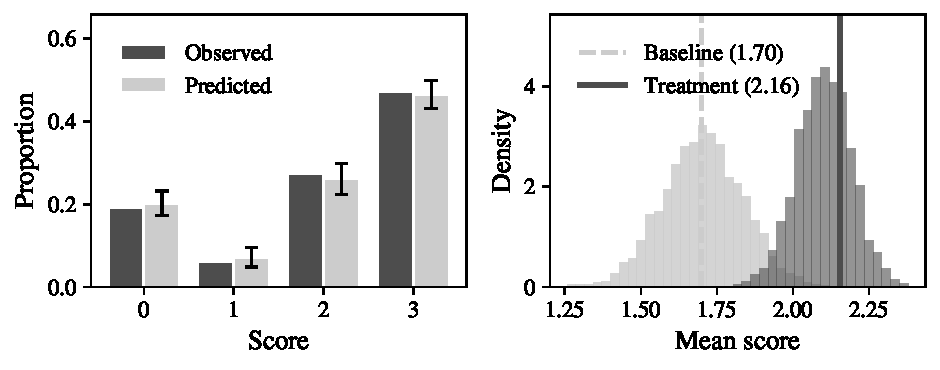
\includegraphics[width=\textwidth]{posterior_predictive_check.pdf}
\caption{} % TODO: PPC; baseline mean 1.70 vs treatment mean 2.16
\label{fig:ppc}
\end{figure}

\subsection{Treatment effect heterogeneity}
% - sigma_beta = 2.11 (94% HDI [1.06, 3.28]); effects -2.36 to +5.44.
% - three groups:
%   BENEFIT (HDI>0): testing_parametrize 5.44 [2.94,8.10];
%     dependencies_module_constants 2.76 [0.60,5.00];
%     architecture_standalone 2.38 [0.29,4.63]. (all near-zero baseline.)
%   MARGINAL NEGATIVE: dependencies_no_new -2.36 [-4.46,-0.03], baseline 2.25 ->
%     treatment 0.77; HEDGE: checker counts re-shown imports -> candidate
%     measurement artifact, not robust harm.
%   NO INTERVENTION (HDI crosses 0): the other 8; high-baseline examples
%     broadcasting 3.00, numpy_style 3.00, snake_no_abbrev 2.67.
\begin{figure}[t]
\centering
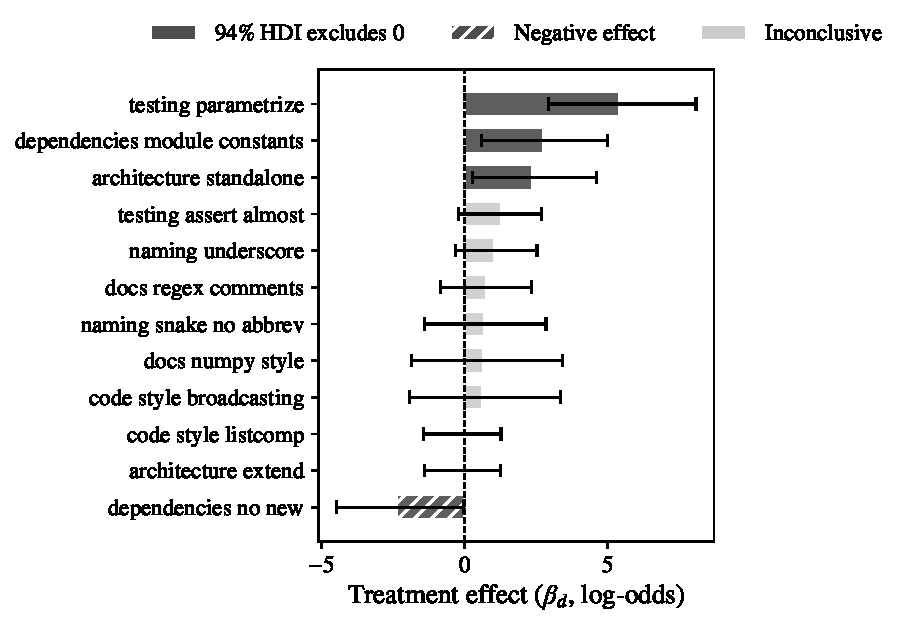
\includegraphics[width=0.85\textwidth]{treatment_effects_forest.pdf}
\caption{} % TODO: per-decision beta forest, 94% HDI
\label{fig:forest}
\end{figure}

\subsection{Model and codebase effects}
% - retention consistent across 5 models (26B-120B for the three with disclosed
%   sizes) and 3 levels of context pressure (98K-203K tokens).
% - HEDGE: baseline from a single model -> per-model retention not fully separable.

\subsection{Reinforcement priorities}
% - gain = delta P(score >= 2) from reinforcement. NOT a closed-loop policy eval;
%   a posterior-derived ranking.
\begin{table}[t]
\centering
\caption{} % TODO caption
\label{tab:policy}
\begin{tabular}{lccl}
\toprule
Decision & Gain & 94\% HDI & Action \\
\midrule
% TODO fill: parametrize +0.78 [+0.46,+0.96] Reinforce;
%   module_constants +0.51 [+0.18,+0.76] Reinforce;
%   arch_standalone +0.34 [+0.06,+0.61] Reinforce;
%   underscore/assert_almost/regex_comments ~+0.14..+0.24 (cross 0) Uncertain;
%   5 other types < +0.04 Skip; deps_no_new -0.47 [-0.77,-0.05] Avoid (marginal).
\bottomrule
\end{tabular}
\end{table}
% - takeaway: only 3 of 12 have gain entirely above zero -> targeted reinforcement.
\begin{figure}[t]
\centering
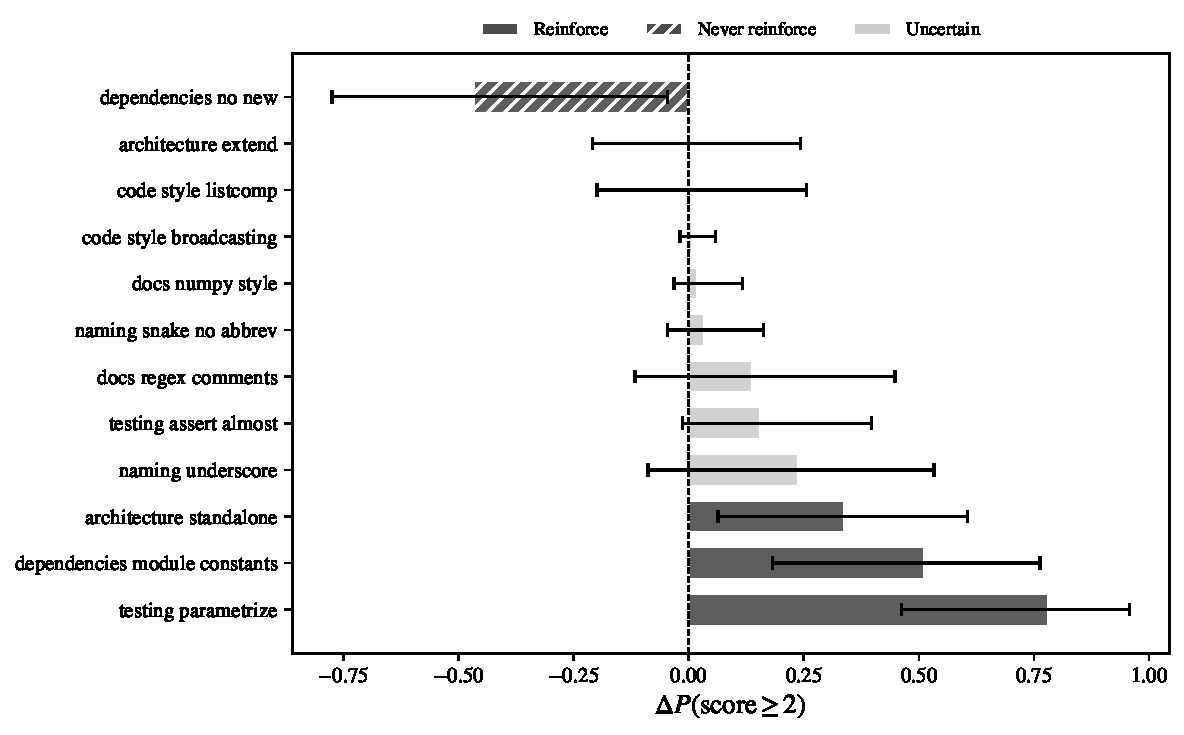
\includegraphics[width=\textwidth]{reinforcement_policy.pdf}
\caption{} % TODO
\label{fig:policy}
\end{figure}

% ---------------------------------------------------------------------
\section{Discussion}
\label{sec:discussion}

\subsection{What determines retention}
% - pattern: instructions the model wouldn't do by default are retained when
%   stated; ones matching default behavior show no effect (winners have near-zero
%   baseline; no-effect ones have baseline ~3.0).
% - deps_no_new is the only negation-phrased one; raise content-vs-framing
%   question; credit the reviewer's paraphrase test (R3) -> future work.

\subsection{Robustness checks}
% - Qwen-only refit (132 of 244): per-decision betas correlate r=0.80 with full;
%   sigma_beta 2.35 vs 2.11. parametrize 6.13, module_constants 2.25,
%   deps_no_new -1.07. architecture_standalone does NOT replicate (-0.71) ->
%   reduce clear winners from 3 to 2.
% - LOO: all Pareto k < 0.7, ELPD = -228.8 +/- 14.5.
\begin{figure}[t]
\centering
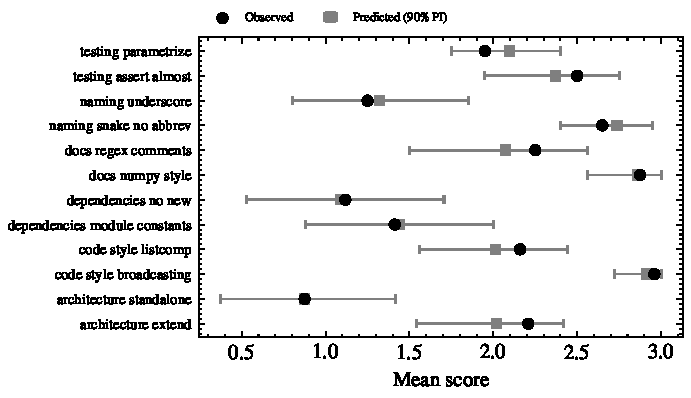
\includegraphics[width=\textwidth]{ppc_per_decision.pdf}
\caption{} % TODO: per-decision PPC
\label{fig:ppc_decision}
\end{figure}

\subsection{Limitations}
% - baseline from one model (Qwen); sensitivity r=0.80 mitigates not eliminates.
% - 244 obs, some cells as small as 4; partial pooling handles it but "uncertain"
%   rankings are preliminary.
% - measured at turns 20-25 only = snapshot, NOT a decay curve; no per-instruction
%   decay rates.
% - checker construct validity: some default to 2; default-2 rates (extend 79%,
%   regex_comments 75%, listcomp 72%, assert_almost 50%); strongest effects have 0%.
% - does NOT implement BKT (tracker not run).

\subsection{Future work}
% - 6 directions: (1) matched baseline+treatment for every model; (2) checker +
%   blinded cross-family LLM-judge panel with agreement (kappa); (3) negated/
%   positive paraphrase test (R3); (4) per-turn scoring -> forgetting curves;
%   (5) closed-loop selective vs uniform under token budget; (6) real coding
%   session traces for ecological validity.

% ---------------------------------------------------------------------
\section{Conclusion}
\label{sec:conclusion}
% - recap: per-instruction retention is heterogeneous; treatment effects span a
%   wide range (state as "nearly eight log-odds units", NOT "order of magnitude").
% - only 3 of 12 worth reinforcing -> targeted not blanket.
% - pattern holds across 5 models, 3 context levels; replicates on single model
%   (r=0.80) with the single-model caveat.
% - BKT loop left to future work.

% ---------------------------------------------------------------------
\subsubsection*{Use of large language models.}
% JAIIO template wording: the author used an LLM (Claude) to improve language and
% readability; results computed by checkers + statistical models, verified by the
% author.

\printbibliography
\end{document}
